% Options for packages loaded elsewhere
\PassOptionsToPackage{unicode}{hyperref}
\PassOptionsToPackage{hyphens}{url}
%
\documentclass[
  ignorenonframetext,
]{beamer}
\usepackage{pgfpages}
\setbeamertemplate{caption}[numbered]
\setbeamertemplate{caption label separator}{: }
\setbeamercolor{caption name}{fg=normal text.fg}
\beamertemplatenavigationsymbolsempty
% Prevent slide breaks in the middle of a paragraph
\widowpenalties 1 10000
\raggedbottom
\setbeamertemplate{part page}{
  \centering
  \begin{beamercolorbox}[sep=16pt,center]{part title}
    \usebeamerfont{part title}\insertpart\par
  \end{beamercolorbox}
}
\setbeamertemplate{section page}{
  \centering
  \begin{beamercolorbox}[sep=12pt,center]{part title}
    \usebeamerfont{section title}\insertsection\par
  \end{beamercolorbox}
}
\setbeamertemplate{subsection page}{
  \centering
  \begin{beamercolorbox}[sep=8pt,center]{part title}
    \usebeamerfont{subsection title}\insertsubsection\par
  \end{beamercolorbox}
}
\AtBeginPart{
  \frame{\partpage}
}
\AtBeginSection{
  \ifbibliography
  \else
    \frame{\sectionpage}
  \fi
}
\AtBeginSubsection{
  \frame{\subsectionpage}
}
\usepackage{lmodern}
\usepackage{amssymb,amsmath}
\usepackage{ifxetex,ifluatex}
\ifnum 0\ifxetex 1\fi\ifluatex 1\fi=0 % if pdftex
  \usepackage[T1]{fontenc}
  \usepackage[utf8]{inputenc}
  \usepackage{textcomp} % provide euro and other symbols
\else % if luatex or xetex
  \usepackage{unicode-math}
  \defaultfontfeatures{Scale=MatchLowercase}
  \defaultfontfeatures[\rmfamily]{Ligatures=TeX,Scale=1}
\fi
\usetheme[]{Singapore}
\usecolortheme{whale}
% Use upquote if available, for straight quotes in verbatim environments
\IfFileExists{upquote.sty}{\usepackage{upquote}}{}
\IfFileExists{microtype.sty}{% use microtype if available
  \usepackage[]{microtype}
  \UseMicrotypeSet[protrusion]{basicmath} % disable protrusion for tt fonts
}{}
\makeatletter
\@ifundefined{KOMAClassName}{% if non-KOMA class
  \IfFileExists{parskip.sty}{%
    \usepackage{parskip}
  }{% else
    \setlength{\parindent}{0pt}
    \setlength{\parskip}{6pt plus 2pt minus 1pt}}
}{% if KOMA class
  \KOMAoptions{parskip=half}}
\makeatother
\usepackage{xcolor}
\IfFileExists{xurl.sty}{\usepackage{xurl}}{} % add URL line breaks if available
\IfFileExists{bookmark.sty}{\usepackage{bookmark}}{\usepackage{hyperref}}
\hypersetup{
  pdftitle={Optimisation via Quantum Computing},
  pdfauthor={Vivek Katial},
  hidelinks,
  pdfcreator={LaTeX via pandoc}}
\urlstyle{same} % disable monospaced font for URLs
\newif\ifbibliography
\setlength{\emergencystretch}{3em} % prevent overfull lines
\providecommand{\tightlist}{%
  \setlength{\itemsep}{0pt}\setlength{\parskip}{0pt}}
\setcounter{secnumdepth}{-\maxdimen} % remove section numbering
\widowpenalties 1 150
\usepackage{amssymb}
\usepackage{amsmath}
\usepackage{amsthm}
\usepackage{braket}
\usepackage{xcolor}

\title{Optimisation via Quantum Computing}
\author{Vivek Katial}
\date{22/01/2020}

\begin{document}
\frame{\titlepage}

\hypertarget{introduction}{%
\section{Introduction}\label{introduction}}

\begin{frame}{About Me}
\protect\hypertarget{about-me}{}

\begin{itemize}
\tightlist
\item
  Vivek Katial
  (\href{mailto:vkatial@student.unimelb.edu.au}{\nolinkurl{vkatial@student.unimelb.edu.au}})

  \begin{itemize}
  \tightlist
  \item
    PhD Candidate (Optimisation on Quantum Computers)
  \end{itemize}
\end{itemize}

\end{frame}

\begin{frame}{Talk Structure}
\protect\hypertarget{talk-structure}{}

\begin{itemize}
\tightlist
\item
  Background
\item
  Proposed Research
\item
  Overview of Literature
\item
  Current Progress
\item
  What's next?
\end{itemize}

\end{frame}

\begin{frame}{Main Research Question}
\protect\hypertarget{main-research-question}{}

\begin{itemize}
\tightlist
\item
  What instances characteristics of optimisation problems make them
  predisposed to being solved on a Quantum Computer?
\end{itemize}

\end{frame}

\hypertarget{background}{%
\section{Background}\label{background}}

\begin{frame}{Adiabatic Quantum Computing (AQC)}
\protect\hypertarget{adiabatic-quantum-computing-aqc}{}

\begin{itemize}[<+->]
\tightlist
\item
  Adiabatic Quantum Computation is a computational model which relies on
  the \emph{adiabatic thereom} of quantum mechanics to compute
  calculations.
\item
  The famous \emph{Schrödinger Equation} is well-known to describe the
  time evolution of a quantum state:
\end{itemize}

\begin{itemize}[<+->]
\tightlist
\item
  \[
  i\hbar \frac{d}{dt} \ket{\psi (t)} = H(t) \ket{\psi(t)}
  \]
\end{itemize}

\begin{itemize}[<+->]
\tightlist
\item
  \(\ket{\psi(t)}\) is our state vector, \(H(t)\) is the time dependent
  Hamiltonian. A Hamiltonian of an \(n\)-qubit system \(H(t)\) is given
  by \(2^n \times 2^n\) matrix.
\end{itemize}

\end{frame}

\begin{frame}{Adiabatic Quantum Computing (AQC)}
\protect\hypertarget{adiabatic-quantum-computing-aqc-1}{}

\begin{itemize}[<+->]
\tightlist
\item
  An adiabatic computation can be expressed by specifying two
  Hamiltonians, denoted by \(H_B\) and \(H_P\) where \(H_B\) is our
  \emph{initial} Hamiltonian and \(H_P\) is the \emph{final} or
  \emph{problem} Hamiltonian.
\item
  \[\begin{matrix}
  H_B &  \xrightarrow{\hspace*{3cm}} & H_P \\
  \ket{\psi_B} &  \text{transform } H(t) &  \ket{\psi_P} \\ 
  \text{known state} &  &  \text{unknown}
  \end{matrix}
  \]
\item
  Loosely speaking, the adiabatic theorem tells us that if we vary from
  \(H_B\) to \(H_P\) \emph{slowly enough} the system will remain in its
  ground state. This fact is a direct result of the Adiabatic Theorem
  {[}1{]}.
\end{itemize}

\end{frame}

\begin{frame}{Adiabatic Quantum Computing (AQC)}
\protect\hypertarget{adiabatic-quantum-computing-aqc-2}{}

\begin{itemize}[<+->]
\tightlist
\item
  To conduct the computation we evolve \(\ket{\psi(t)}\) till time
  \(t=T\) such that \(\ket{\psi(t=T)}\) encodes the answer. The
  computation is done using a Hamiltonian which linearly interpolates
  between \(H_B\) and \(H_P\). Specifically as below:
\end{itemize}

\begin{itemize}[<+->]
\tightlist
\item
  \[
  H(t) = \left(1 - \frac{t}{T}\right)H_B + \frac{t}{T}H_P
  \]
\item
  How fast?
\item
  \[
  T =  \frac{1}{\min_t  g(t)^2}
  \]
\item
  Where \(g(t)\) is the difference between the first two smallest
  eigenvalues of \(H(t)\)
\end{itemize}

\end{frame}

\begin{frame}{3SAT (Exact Cover)}
\protect\hypertarget{sat-exact-cover}{}

\begin{itemize}[<+->]
\tightlist
\item
  The satisfiability problem, abbreviated SAT, is a classic example of
  an NP-complete problem {[}2{]}
\item
  The basic SAT formulation can be described as follows: Given a boolean
  formula (AND \(\land\), OR \(\lor\) , NOT \(\neg\)) over \(n\)
  variables (\(z_1, z_2, ... , z_n\)). Can one set \(z_i\)'s in a manner
  such that the Boolean formula is true?
\item
  A clause is an expression which the variables must satisfy. For
  example \(z_1 \land z_2 \implies z_1 = z_2 = 1\)
\end{itemize}

\end{frame}

\begin{frame}{3SAT (Exact Cover Example)}
\protect\hypertarget{sat-exact-cover-example}{}

\begin{itemize}[<+->]
\tightlist
\item
  Consider a 4-bit number with two clauses:

  \begin{itemize}[<+->]
  \tightlist
  \item
    \(z_1 \land z_2 \land z_3\)
  \item
    \(z_1 \land z_3 \land z_4\)
  \end{itemize}
\item
  Here we have 16 possible assignments, namely:
\item
  \begin{align*}
  \mathcal{Z} = \{\,
  & 0000, 0001, 0010, 0011, 0100, 0101, 0110, 0111, \\
  & 1000, 1001, 1010, 1011, 1100, 1101, 1110, 1111 \,\}\enspace
  \end{align*}
\end{itemize}

\begin{itemize}[<+->]
\tightlist
\item
  However, our \textbf{satisfying assignment} is only \(\vec{z} = 1111\)
\end{itemize}

\end{frame}

\begin{frame}{Mapping 3SAT to AQC}
\protect\hypertarget{mapping-3sat-to-aqc}{}

\begin{itemize}[<+->]
\tightlist
\item
  How do we construct \(H_B\) and \(H_P\) so that we can solve our
  optimisation problem?
\item
  Farhi et al.{[}3{]} describe this construction in considerable detail.
\item
  We then evolve our system with the following interpolation:
\item
  \[
  H(t) = \left(1 - \frac{t}{T}\right)H_B + \frac{t}{T}H_P
  \]
\item
  Finally, complete measurement and our solution is our final state
  \(\ket{\psi(t=T)}\)
\end{itemize}

\end{frame}

\begin{frame}{Proposed Research}
\protect\hypertarget{proposed-research}{}

\begin{itemize}[<+->]
\tightlist
\item
  Depending on different structures of instances, classical algorithms
  may perform differently to Quantum ones.
\item
  We are looking to investigate which types of instances are more
  pre-disposed to being solved on Quantum Computers:
\item
  To do this we have simulated AQC and probe the ``quantumness'' of each
  instance:

  \begin{enumerate}[<+->]
  \tightlist
  \item
    Minimum Energy Gap \(g_{\text{min}}\)
  \item
    Entropy of Entanglement
  \end{enumerate}
\end{itemize}

\end{frame}

\begin{frame}{Proposed Research}
\protect\hypertarget{proposed-research-1}{}

\begin{itemize}[<+->]
\tightlist
\item
  This will involve large amounts of generating experimental data
\item
  To survey the instances we will deploy the instance space analysis
  methodology {[}4--6{]}
\item
  Ultimately, we can build a prediction model which maps instance
  features of different 3SAT instances to their inherent ``Quantumness''
\end{itemize}

\end{frame}

\begin{frame}{Proposed Research}
\protect\hypertarget{proposed-research-2}{}

\begin{itemize}[<+->]
\tightlist
\item
  Given that we have access to IBM's Quantum Computer, we can also use
  this approach on QAOA and produce results from a \emph{universal
  quantum computer}.
\item
  This methodology can then be further extended to other optimisation
  problems that can be mapped to Quadratic Unconstrained Binary
  Optimisation (QUBO) problems.
\end{itemize}

\end{frame}

\begin{frame}{Algorithm Selection}
\protect\hypertarget{algorithm-selection}{}

\begin{itemize}[<+->]
\tightlist
\item
  Given a set of problem instances, predicting which algorithm is most
  likely to best perform was first explored by Rice {[}7{]}. \pause
\end{itemize}

\begin{center}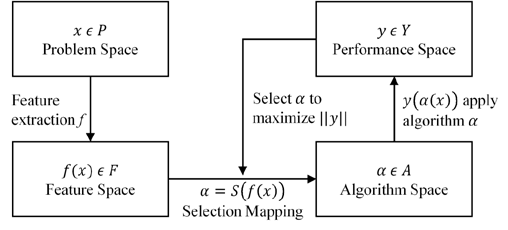
\includegraphics[width=0.6\linewidth]{./rices-framework-for-algorithm-selection} \end{center}

\begin{itemize}[<+->]
\tightlist
\item
  However, what we are interested in is probing the strengths and
  weaknesses of AQC for different instances of SAT.
\end{itemize}

\end{frame}

\begin{frame}{Instance Space Methodology}
\protect\hypertarget{instance-space-methodology}{}

\begin{itemize}[<+->]
\tightlist
\item
  The instance space methodology presented in {[}4--6{]} extends Rice's
  framework. \pause
\end{itemize}

\begin{center}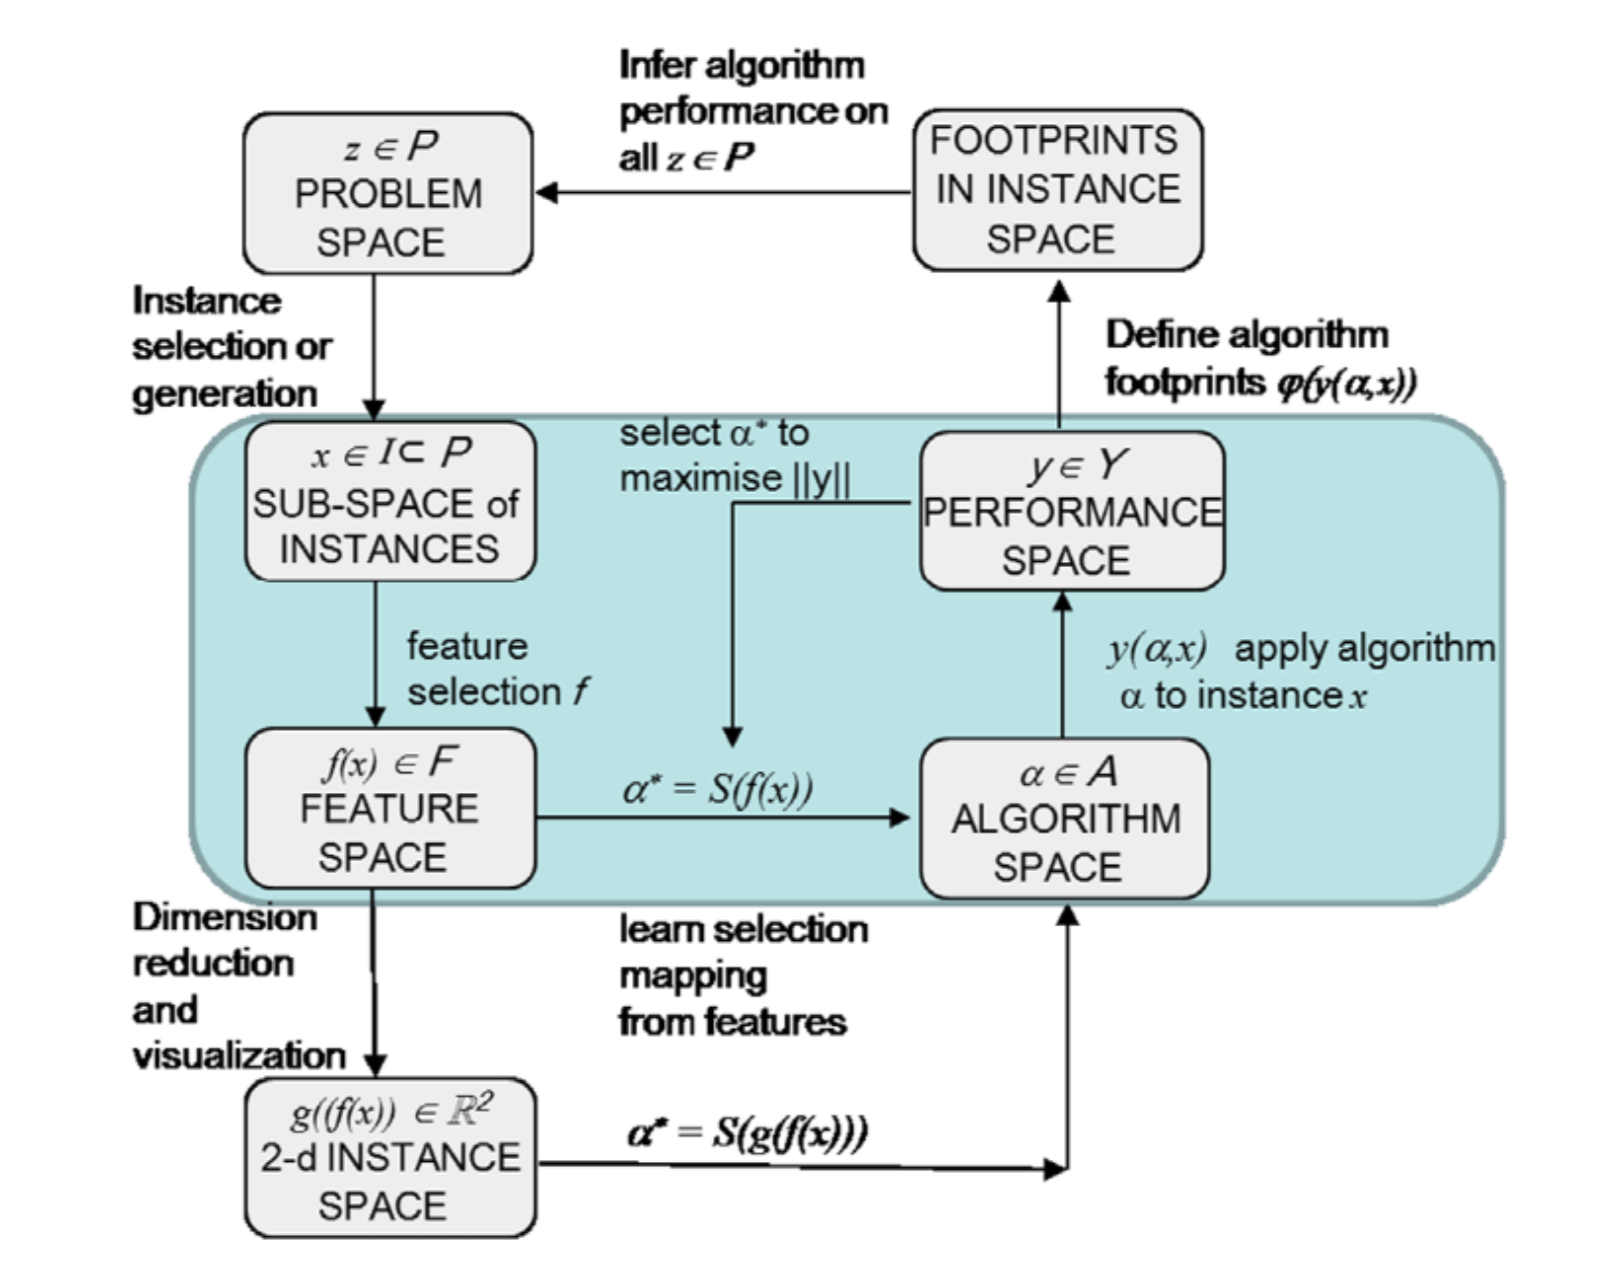
\includegraphics[width=0.6\linewidth]{./instance-space-methodology} \end{center}

\end{frame}

\begin{frame}{Instance Space Methodology}
\protect\hypertarget{instance-space-methodology-1}{}

\begin{center}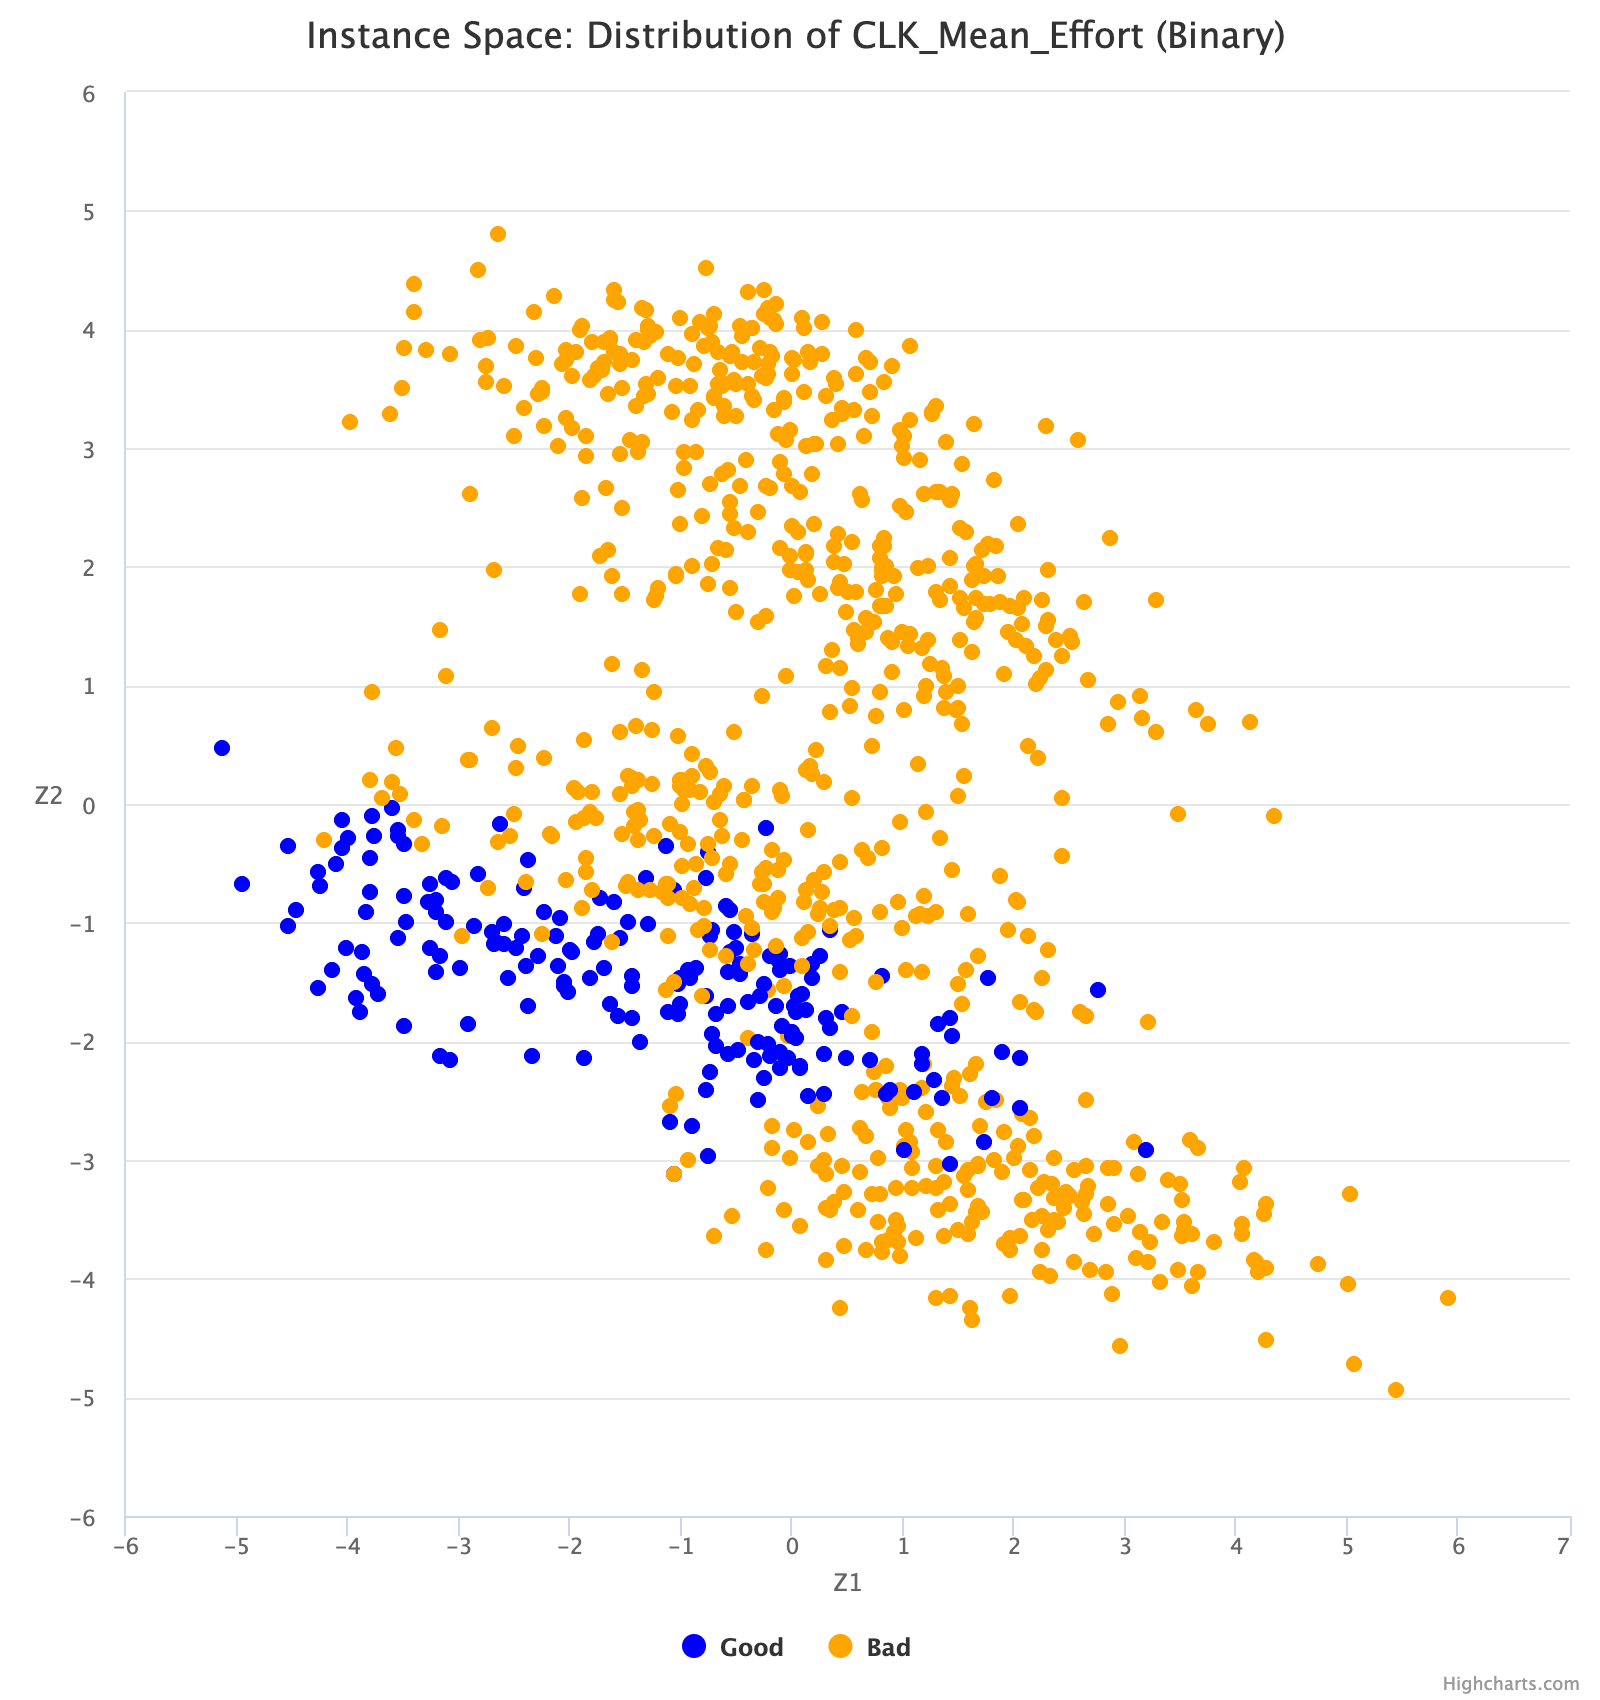
\includegraphics[width=0.6\linewidth]{./Performance-distribution-binary} \end{center}

\end{frame}

\begin{frame}{Instance Space Methodology}
\protect\hypertarget{instance-space-methodology-2}{}

\begin{center}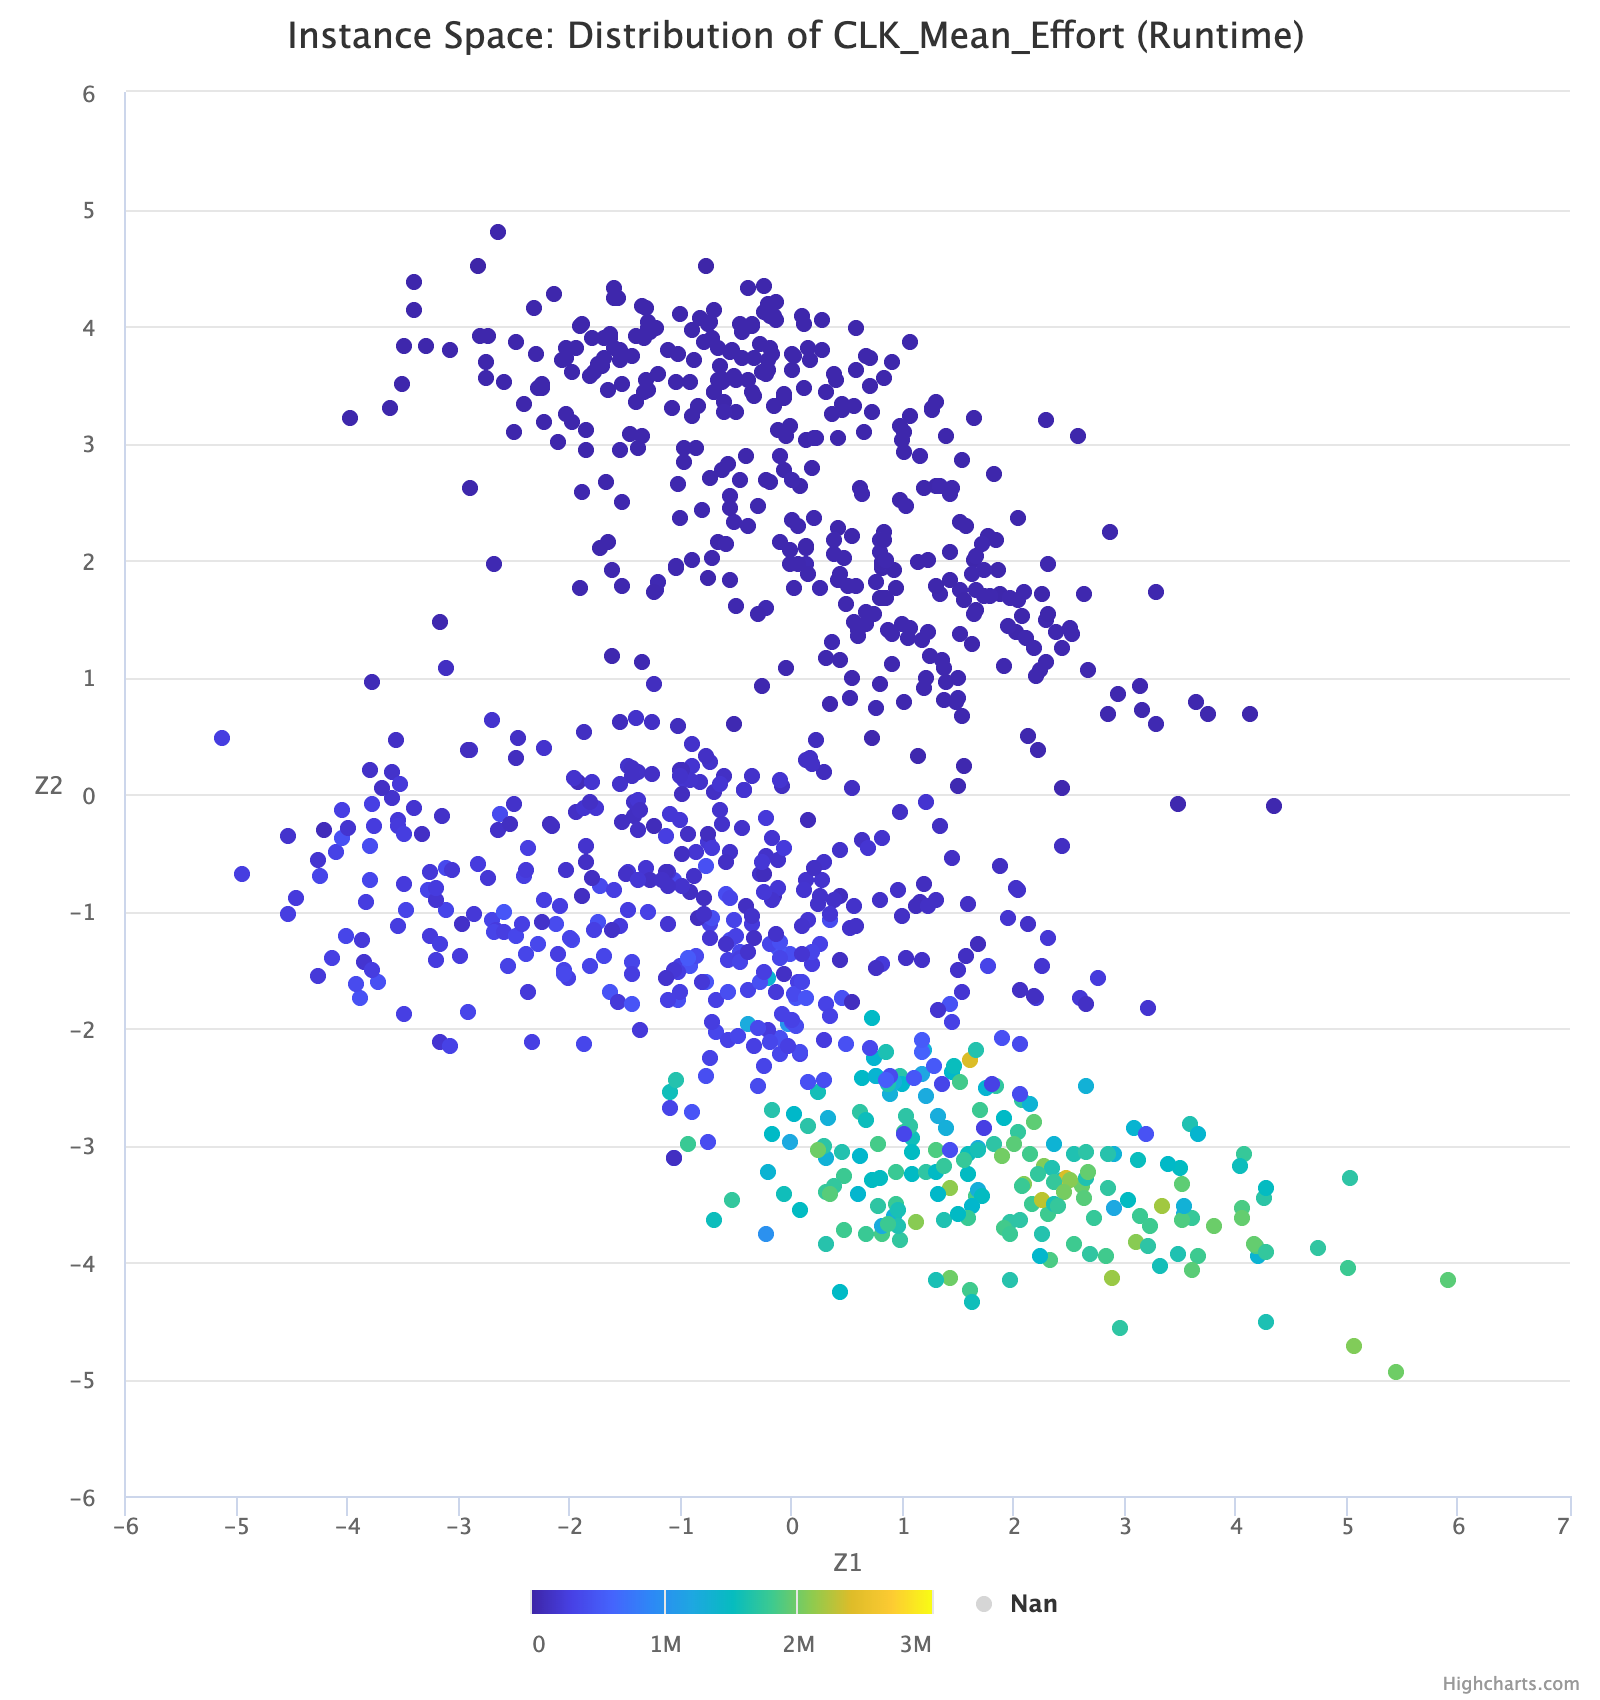
\includegraphics[width=0.6\linewidth]{./Performance-distribution} \end{center}

\end{frame}

\begin{frame}{Hardness Features for 3SAT}
\protect\hypertarget{hardness-features-for-3sat}{}

\begin{itemize}[<+->]
\tightlist
\item
  Selman et. al demonstrated {[}8{]} the existence of a phase transition
  for random 3SAT problems.
\item
  SATZilla and Nudelman et. al have identified 84 different features for
  SAT instances {[}9,10{]}.
\end{itemize}

\pause

\begin{columns}[T]
\begin{column}{0.5\textwidth}
\small

\begin{enumerate}
\tightlist
\item
  Problem Size Features
\item
  Variable-Clause Graph Features
\item
  Variable Graph Features
\item
  Clause Graph Features
\item
  Proximity to Horn Formula
\end{enumerate}
\end{column}

\begin{column}{0.5\textwidth}
\pause
\small

\begin{enumerate}
\setcounter{enumi}{5}
\tightlist
\item
  Balance Features
\item
  DPLL Probing Features
\item
  Local Search Probing Features
\item
  LP-Based Features
\end{enumerate}
\end{column}
\end{columns}

\end{frame}

\begin{frame}{Quantum Computing Research into Hard SAT problems}
\protect\hypertarget{quantum-computing-research-into-hard-sat-problems}{}

\begin{itemize}[<+->]
\tightlist
\item
  In their seminal paper {[}3{]} Farhi et al.~aswell as Hogg et
  al.~{[}11{]} touched on the phase transition and showed that the
  minimum energy gap perhaps scaled polynomially with \(n\) as roughly
  \(N^2\).
\item
  However in 2009, Young et al {[}12{]}. demonstrated via monte-carlo
  simulations of \(N=256\) that some USA instances have a \emph{quantum
  phase transition}.
\item
  Their research indicated that as \(N \rightarrow \infty\) the system
  is expected to lead to an exponentially small gap, and hence an
  exponential complexity.
\item
  Farhi et al.~{[}13{]} also investigated different evolution paths and
  their results suggested it is possible to overcome the exponentially
  small minimum gap by selecting random initial Hamiltonians
\end{itemize}

\end{frame}

\begin{frame}{Quantum Computing Research into Hard SAT problems}
\protect\hypertarget{quantum-computing-research-into-hard-sat-problems-1}{}

\begin{itemize}[<+->]
\tightlist
\item
  Latorre et al.~probed the entropy of entanglement for 250 USA
  Instances of Exact-Cover {[}14{]}, their results showed that entropy
  of entanglement scales linearly with \(N\).
\item
  However, their results also showed that for large \(N\), the minimum
  gap scaling is exponential and can be associated with a \emph{quantum
  phase transition} {[}14{]}.
\item
  Hauke et al.~{[}15{]} ran simulations of adiabatic quantum
  optimisation with \(n=16\). Their results indicated that large
  entanglement entropy has little significance for the success
  probability of the optimisation task.
\end{itemize}

\end{frame}

\begin{frame}{Quantum Computing Research into Hard SAT problems}
\protect\hypertarget{quantum-computing-research-into-hard-sat-problems-2}{}

\begin{itemize}[<+->]
\tightlist
\item
  Choi et al.~{[}16{]} showed that problem Hamiltonian parameters can
  affect the minimum spectral gap of AQC.
\item
  Gabor et al.~{[}17{]} shows that the phase transition from 3SAT
  persists in some form (but possibly to a lesser extent) in AQC via
  \textbf{real experimental results} on D-WAVE.
\item
  Most signficant for us is that none of this work approaches instances
  in a robust manner such as the MATILDA framework
\end{itemize}

\end{frame}

\begin{frame}{Current Progress}
\protect\hypertarget{current-progress}{}

\begin{enumerate}[<+->]
\tightlist
\item
  Learning Quantum Mechanics and Quantum Computing
\item
  Conducting literature review on current advances in Adiabatic Quantum
  Computing.
\item
  Developed working environment, set up GitHub, scripts, organizational
  tools enabling an efficient working environment.
\end{enumerate}

\end{frame}

\begin{frame}{Current Progress}
\protect\hypertarget{current-progress-1}{}

\begin{enumerate}[<+->]
\setcounter{enumi}{3}
\tightlist
\item
  Developed an architecture to run reproducible experiments at scale
\item
  Provisioned all infrastructure required for above on Melbourne
  Research Cloud and SPARTAN
\item
  Developed a working implementation of Adiabatic Quantum Computing on
  different instances of 3SAT.
\end{enumerate}

\end{frame}

\begin{frame}{Next Steps (untill Confirmation)}
\protect\hypertarget{next-steps-untill-confirmation}{}

\begin{enumerate}[<+->]
\tightlist
\item
  Complete Literature Review of current advances in AQC.
\item
  Implement scripts to generate \textbf{hard} instances of 3SAT with
  respect to \emph{instance characteristics}.
\item
  Apply Instance Space Methodology from MATILDA to find decision
  boundaries for \emph{Entanglement Entropy} and \emph{Minimum Energy
  Gap}
\end{enumerate}

\end{frame}

\begin{frame}[fragile]{Next Steps (untill Confirmation)}
\protect\hypertarget{next-steps-untill-confirmation-1}{}

\begin{enumerate}[<+->]
\setcounter{enumi}{3}
\tightlist
\item
  Extend implementation to work on QAOA and VQE with \texttt{QisKit}
\item
  Learn C++ effectively, this will be required when implementing larger
  simulations.
\item
  Apply Tensor Network methodology on current simulations
\item
  Further advance knowledge of Quantum Physics (possibly through taking
  a course in Quantum Computing)
\item
  Extend research to look at other optimisation problems
\end{enumerate}

\end{frame}

\hypertarget{references}{%
\section{References}\label{references}}

\begin{frame}[allowframebreaks]{References}
\protect\hypertarget{references-1}{}

\small

\hypertarget{refs}{}
\leavevmode\hypertarget{ref-Born1928}{}%
1. Born M, Fock V (1928) Beweis des adiabatensatzes. \emph{Zeitschrift
für Physik} 51: 165--180.

\leavevmode\hypertarget{ref-Cook1971}{}%
2. Cook SA (1971) The complexity of theorem-proving procedures, In,
\emph{Proceedings of the third annual acm symposium on theory of
computing}, ACM, 151--158.

\leavevmode\hypertarget{ref-Farhi2001}{}%
3. Farhi E, Goldstone J, Gutmann S, et al. (2001) A quantum adiabatic
evolution algorithm applied to random instances of an np-complete
problem. \emph{Science} 292: 472--475.

\leavevmode\hypertarget{ref-Smith-Miles2015}{}%
4. Smith-Miles K, Bowly S (2015) Generating new test instances by
evolving in instance space. \emph{Computers \& Operations Research} 63:
102--113.

\leavevmode\hypertarget{ref-Smith-Miles2012}{}%
5. Smith-Miles K, Lopes L (2012) Measuring instance difficulty for
combinatorial optimization problems. \emph{Computers \& Operations
Research} 39: 875--889.

\leavevmode\hypertarget{ref-Smith-Miles2014}{}%
6. Smith-Miles K, Baatar D, Wreford B, et al. (2014) Towards objective
measures of algorithm performance across instance space. \emph{Computers
\& Operations Research} 45: 12--24.

\leavevmode\hypertarget{ref-Rice1976}{}%
7. Rice JR, others (1976) The algorithm selection problem.
\emph{Advances in computers} 15: 5.

\leavevmode\hypertarget{ref-Selman1996}{}%
8. Selman B, Mitchell DG, Levesque HJ (1996) Generating hard
satisfiability problems. \emph{Artificial Intelligence} 81: 17--29.

\leavevmode\hypertarget{ref-Xu2008}{}%
9. Xu L, Hutter F, Hoos HH, et al. (2008) SATzilla: Portfolio-based
algorithm selection for sat. \emph{Journal of artificial intelligence
research} 32: 565--606.

\leavevmode\hypertarget{ref-Nudelman2004}{}%
10. Nudelman E, Leyton-Brown K, Hoos HH, et al. (2004) Understanding
random sat: Beyond the clauses-to-variables ratio, In: Wallace M (Ed.),
\emph{Principles and practice of constraint programming -- cp 2004},
Berlin, Heidelberg, Springer Berlin Heidelberg, 438--452.

\leavevmode\hypertarget{ref-Hogg2002}{}%
11. Hogg T (2002) Adiabatic quantum computing for random satisfiability
problems. \emph{Phys Rev A 67 022314 (2003)}.

\leavevmode\hypertarget{ref-Young2009}{}%
12. Young AP, Knysh S, Smelyanskiy VN (2009) First order phase
transition in the quantum adiabatic algorithm. \emph{Phys Rev Lett 104,
020502 (2010)}.

\leavevmode\hypertarget{ref-Farhi2009}{}%
13. Farhi E, Goldstone J, Gosset D, et al. (2009) Quantum adiabatic
algorithms, small gaps, and different paths. \emph{arXiv preprint
arXiv:09094766}.

\leavevmode\hypertarget{ref-Latorre2004}{}%
14. Latorre JI, Orús R (2004) Adiabatic quantum computation and quantum
phase transitions. \emph{Physical Review A} 69: 062302.

\leavevmode\hypertarget{ref-Hauke2015}{}%
15. Hauke P, Bonnes L, Heyl M, et al. (2015) Probing entanglement in
adiabatic quantum optimization with trapped ions. \emph{Frontiers in
Physics} 3: 21.

\leavevmode\hypertarget{ref-Choi2020}{}%
16. Choi V (2020) The effects of the problem hamiltonian parameters on
the minimum spectral gap in adiabatic quantum optimization.
\emph{Quantum Information Processing} 19: 90.

\leavevmode\hypertarget{ref-Gabor2019}{}%
17. Gabor T, Zielinski S, Feld S, et al. (2019) Assessing solution
quality of 3SAT on a quantum annealing platform, In, \emph{International
workshop on quantum technology and optimization problems}, Springer,
23--35.

\end{frame}

\end{document}
